% ---------------------------------------------------------------------------
% Author guideline and sample document for EG publication using LaTeX2e input
% D.Fellner, v1.15, Dec 14, 2018

\documentclass{egpubl}
\usepackage{EGVMV19}

% --- for  Annual CONFERENCE
% \ConferenceSubmission   % uncomment for Conference submission
% \ConferencePaper        % uncomment for (final) Conference Paper
% \STAR                   % uncomment for STAR contribution
% \Tutorial               % uncomment for Tutorial contribution
% \ShortPresentation      % uncomment for (final) Short Conference Presentation
% \Areas                  % uncomment for Areas contribution
% \MedicalPrize           % uncomment for Medical Prize contribution
% \Education              % uncomment for Education contribution
% \Poster                 % uncomment for Poster contribution
% \DC                     % uncomment for Doctoral Consortium
%
% --- for  CGF Journal
% \JournalSubmission    % uncomment for submission to Computer Graphics Forum
% \JournalPaper         % uncomment for final version of Journal Paper
%
% --- for  CGF Journal: special issue
% \SpecialIssueSubmission    % uncomment for submission to , special issue
% \SpecialIssuePaper         % uncomment for final version of Computer Graphics Forum, special issue
%                          % EuroVis, SGP, Rendering, PG
% --- for  EG Workshop Proceedings
 \WsSubmission      % uncomment for submission to EG Workshop
% \WsPaper           % uncomment for final version of EG Workshop contribution
% \WsSubmissionJoint % for joint events, for example ICAT-EGVE
% \WsPaperJoint      % for joint events, for example ICAT-EGVE
% \Expressive        % for SBIM, CAe, NPAR
% \DigitalHeritagePaper
% \PaperL2P          % for events EG only asks for License to Publish

% --- for EuroVis
% for full papers use \SpecialIssuePaper
% \STAREurovis   % for EuroVis additional material
% \EuroVisPoster % for EuroVis additional material
% \EuroVisShort  % for EuroVis additional material

% !! *please* don't change anything above
% !! unless you REALLY know what you are doing
% ------------------------------------------------------------------------
\usepackage[T1]{fontenc}
\usepackage{dfadobe}

\usepackage{cite}  % comment out for biblatex with backend=biber
% ---------------------------
%\biberVersion
\BibtexOrBiblatex
%\usepackage[backend=biber,bibstyle=EG,citestyle=alphabetic,backref=true]{biblatex}
%\addbibresource{egbibsample.bib}
% ---------------------------
\electronicVersion
\PrintedOrElectronic
% for including postscript figures
% mind: package option 'draft' will replace PS figure by a filename within a frame
\ifpdf \usepackage[pdftex]{graphicx} \pdfcompresslevel=9
\else \usepackage[dvips]{graphicx} \fi

\usepackage{egweblnk}


\usepackage{times}
\usepackage{epsfig}
\usepackage{graphicx}
\usepackage{amsmath}
\usepackage{amssymb}

% Include other packages here, before hyperref.
\usepackage{algorithm}
\usepackage{algpseudocode}
\usepackage{wrapfig}
\usepackage{subcaption}

\usepackage{caption}
\captionsetup[table]{position=bottom}

\usepackage{array}
\usepackage{epstopdf}
\usepackage{cuted}
\begingroup
  \catcode`\_=\active
  \gdef_#1{\ensuremath{\sb{\mathrm{#1}}}}
\endgroup
\mathcode`\_=\string"8000
\catcode`\_=12

\usepackage{xcolor}
\usepackage{textcomp}
\definecolor{Gray}{rgb}{0.5,0.5,0.5}
\definecolor{darkblue}{rgb}{0,0,0.7}
\definecolor{orange}{rgb}{1,.5,0} % something readable but different from todo
\definecolor{red}{rgb}{1,0,0} % something readable but different from todo
\newcommand{\heading}[1]{\noindent\textbf{#1}}
\newcommand{\note}[1]{{\em{\textcolor{orange}{#1}}}}
\newcommand{\todo}[1]{{\textcolor{darkblue}{TODO: #1}}}
\newcommand{\changed}[1]{{\textcolor{blue}{#1}}}

\newcommand{\Matrix}[1]     {{\ensuremath{\mathbf{\uppercase{#1}}}}} %Matrix 
\newcommand{\Vector}[1]     {{\ensuremath{\mathbf{\lowercase{#1}}}}} %Vector
\newcommand{\Variable}[1]   {{\ensuremath{\mathrm{\lowercase{#1}}}}} %Scalar
\newcommand{\Id}            {\mathbb{I}} %Identity matrix

\newcommand{\mini}[1]   {\underset{{#1}}{\operatorname{min}} \: \: } %Minimize w.r.t.
\newcommand{\minimize}[1]   {\underset{{#1}}{\operatorname{argmin}} \: \: } %Minimize w.r.t.
\newcommand{\subjectto}     {\operatorname{subject to}}

\newcommand{\signal} {\Vector{x}}
\newcommand{\filter} {\Vector{d}}
\newcommand{\code}   {\Vector{z}}
\newcommand{\Filter} {\Matrix{D}}
\newcommand{\mask}   {\Matrix{M}}
\newcommand{\Code}   {\Matrix{z}}
\newcommand{\surC}   {\Matrix{C}}
\newcommand{\surB}   {\Matrix{B}}
\newcommand{\matA}   {\Matrix{A}}
\newcommand{\ite}	 {t}

% ---------------------------------------------------------------------
% end of prologue

% EG author guidelines plus sample file for EG publication using LaTeX2e input
% D.Fellner, v2.03, Dec 14, 2018


\title{Stochastic Convolutional Sparse Coding \\
        Supplementary Material}

% for anonymous conference submission please enter your SUBMISSION ID
% instead of the author's name (and leave the affiliation blank) !!
% for final version: please provide your *own* ORCID in the brackets following \orcid; see https://orcid.org/ for more details.
\author{Submission ID: 1010}
%\author[D. Fellner \& S. Behnke]
%{\parbox{\textwidth}{\centering D.\,W. Fellner\thanks{Chairman Eurographics Publications Board}$^{1,2}$\orcid{0000-0001-7756-0901}
%        and S. Behnke$^{2}$\orcid{0000-0001-5923-423X}
%%        S. Spencer$^2$\thanks{Chairman Siggraph Publications Board}
%        }
%        \\
%% For Computer Graphics Forum: Please use the abbreviation of your first name.
%{\parbox{\textwidth}{\centering $^1$TU Darmstadt \& Fraunhofer IGD, Germany\\
%         $^2$Graz University of Technology, Institute of Computer Graphics and Knowledge Visualization, Austria
%%        $^2$ Another Department to illustrate the use in papers from authors
%%             with different affiliations
%       }
%}
%}
% ------------------------------------------------------------------------

% if the Editors-in-Chief have given you the data, you may uncomment
% the following five lines and insert it here
%
% \volume{36}   % the volume in which the issue will be published;
% \issue{1}     % the issue number of the publication
% \pStartPage{1}      % set starting page


%-------------------------------------------------------------------------
\begin{document}

% uncomment for using teaser
% \teaser{
%  \includegraphics[width=\linewidth]{eg_new}
%  \centering
%   \caption{New EG Logo}
% \label{fig:teaser}
%}

\maketitle
%-------------------------------------------------------------------------
\section{Solvers for LASSO and QCQP}
Algorithm~\ref{algo:ADMMLasso} is used to optimize a LASSO problem in the following form:
\begin{equation}
    \minimize{\code} \frac{1}{2}\|\signal - \Filter \code \|_2^2 + \lambda\| \code \|_1
\end{equation}

\begin{algorithm}
\caption{ADMM framework for solving LASSO} \label{algo:ADMMLasso}
\begin{algorithmic}[1]
    \For{$s=1$ to $S$}
        \State // z-update step (quadratic programming)
        \State $\code^{s+1} \gets (\Filter ^ \top \Filter + \rho \Id )^{-1}(\Filter^\top \signal + \rho(\Vector{y}^s - \Vector{q}^s ) )$
        \State // y-update step (soft thresholding)
        \State $\Vector{y}^{s+1} \gets (\code^{s+1}+\Vector{q}^{s} - \frac{\lambda}{\rho})_{+} ~ - ~ (-\code^{s+1}-\Vector{q}^{s} - \frac{\lambda}{\rho})_{+}$
        \State // scaled dual variables update
        \State $\Vector{q}^{s+1} \gets \bold{q}^{s}+\code^{s+1}-\Vector{y}^{s+1}$
    \EndFor
\end{algorithmic}
\end{algorithm}
$S$ is the total number of ADMM iteration. $\Vector{y}$ is the introduced slack variable, $\Vector{q}$ is the scaled dual variable, and $\rho$ is the augmented Lagrangian penalty.

\begin{algorithm}
\caption{Projected Block Coordinate Descent for solving QCQP} \label{algo:BCDQCQP}
\begin{algorithmic}[1]
\State $\Vector{r} \gets \signal - \Code \filter $
\While {not converge}
    \For{$k=1$ to $K$}
        \State $ \filter^{\ast}_k \gets \filter_k + \Code_k ^ \top \Vector{r} ~ / ~ L_k $
        \State $ \filter^{\ast}_k \gets \filter^{\ast}_k ~ / ~ \text{max}( \|\filter^{\ast}_k\|,1 ) $
        \State $ \Vector{r} ~~ \gets \Vector{r} + \Code_k( \filter_k - \filter^{\ast}_k ) $
    \EndFor
    \State  $ \filter \gets \filter^{\ast} $
\EndWhile
\end{algorithmic}
\end{algorithm}


Algorithm~\ref{algo:BCDQCQP} is used to optimize a QCQP problem in the following form:
\begin{equation}
\begin{split}
    \minimize{\filter} & \frac{1}{2}\|\signal - \Code \filter \|_2^2 \\
    \text{subject to} & ~ \|\filter_k\|^2_2 \leq 1 ~~ \forall k \in \{1,\dots,K\},
\end{split}
\end{equation}

$L_k$ is the Lipschitz constant of $\Code_k^\top \Code_k$.

\section{Additional Experiments}

\begin{figure}[h]
\begin{subfigure}{0.45\textwidth}
  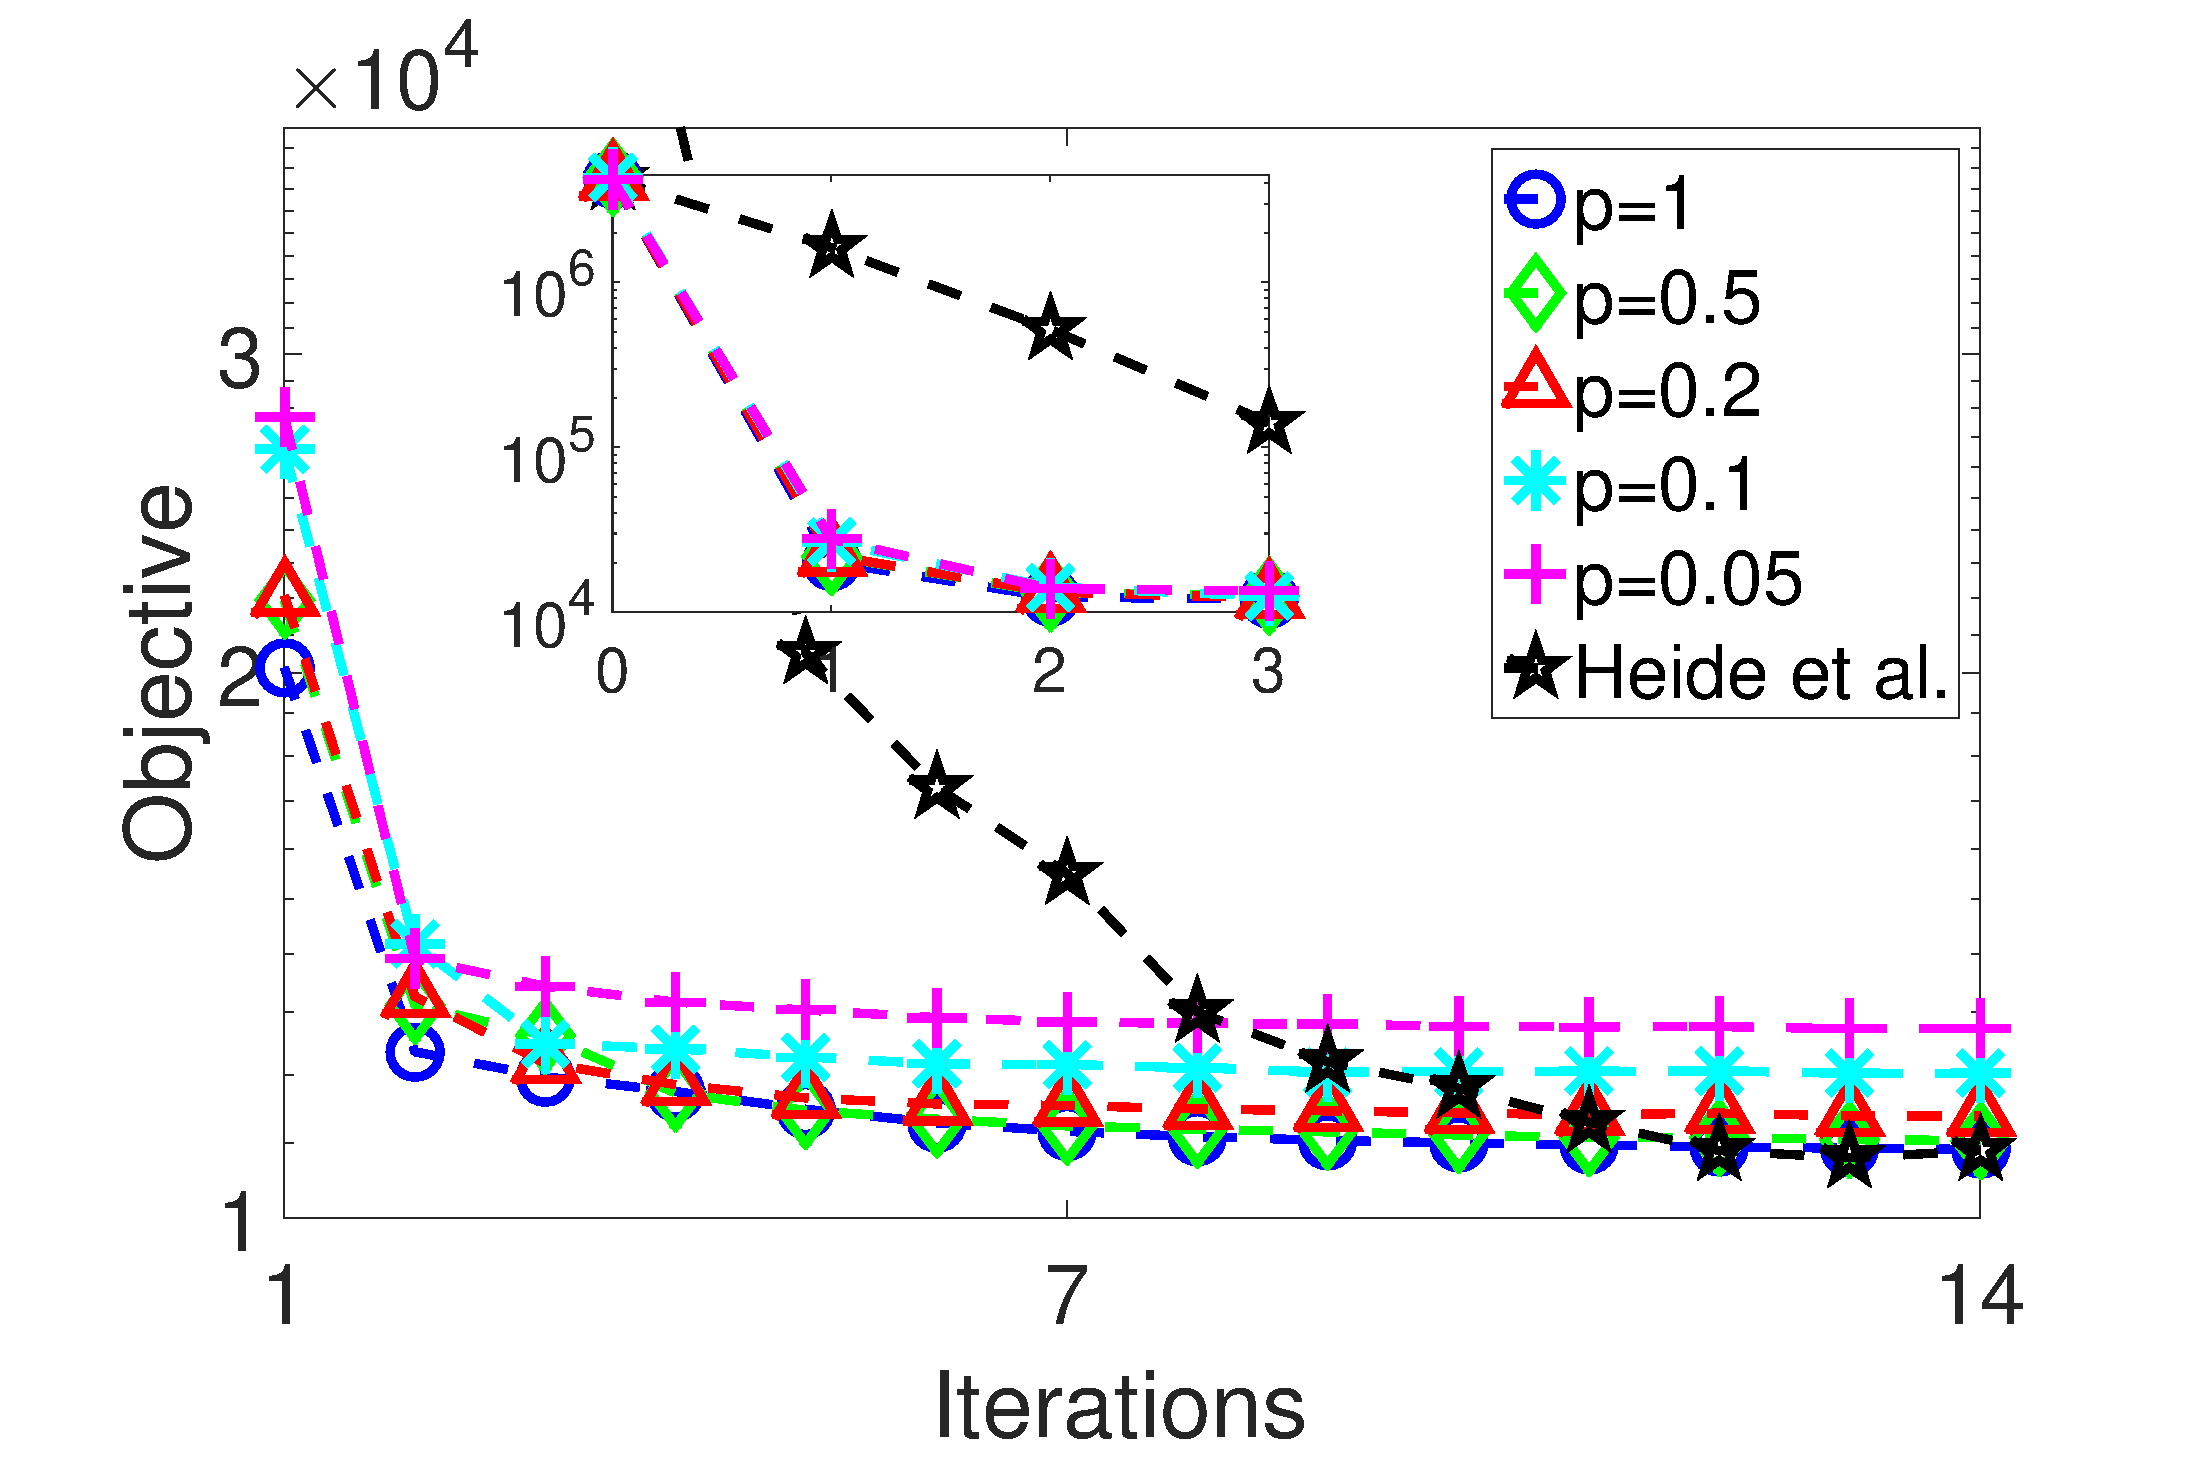
\includegraphics[width=1\linewidth]{figure/iteVSobj-city.pdf}
\end{subfigure}
\begin{subfigure}{0.45\textwidth}
  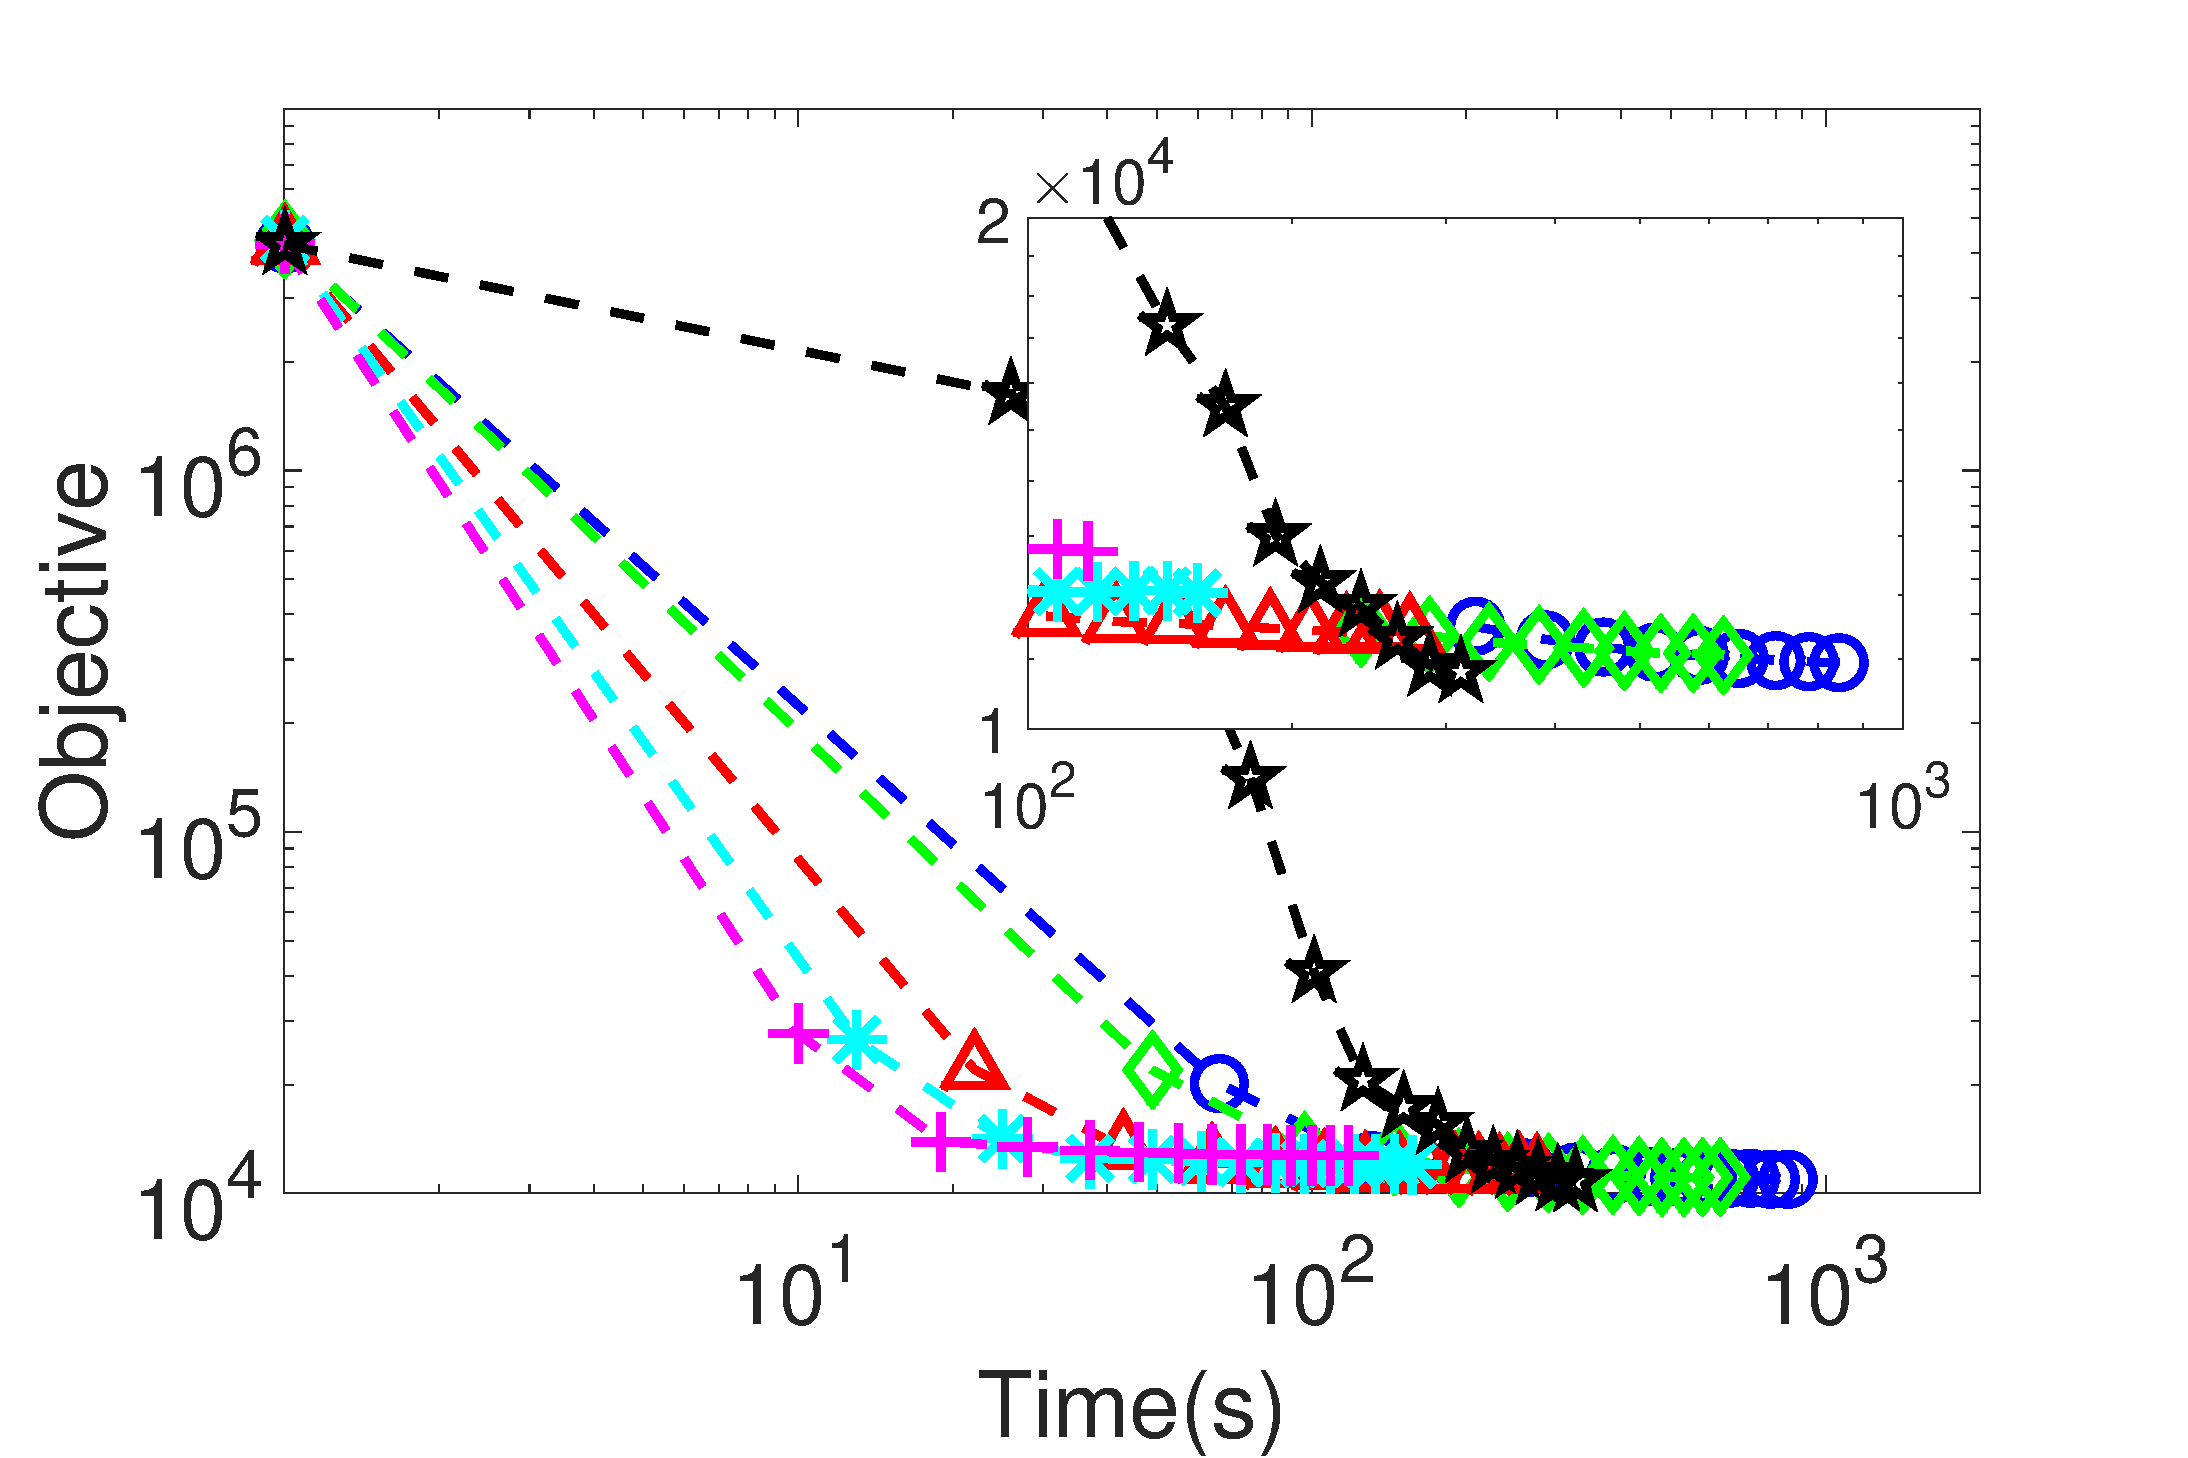
\includegraphics[width=1\linewidth]{figure/timeVSobj-city.pdf}
\end{subfigure}

\caption{Experimental results obtained on the city dataset. Convergence comparison between the-state-of-art batch method and SBCSC with different subsampling probability.}
\label{fig:subsampleResult-city}
\end{figure}

In order to show the robustness of the proposed algorithms, We also conduct experiments on city dataset. We first compare SBCSC with the state-of-the-art batch-mode algorithm, and the results are shown in Fig.\ \ref{fig:subsampleResult-city}. Similar to the results shown in Fig.~1 in the main manuscript, SBCSC, with $p=0.1$, outperforms the compared batch-mode algorithm in terms of runtime performance. 

\begin{figure}[h]
\centering
\begin{subfigure}{0.45\textwidth}
  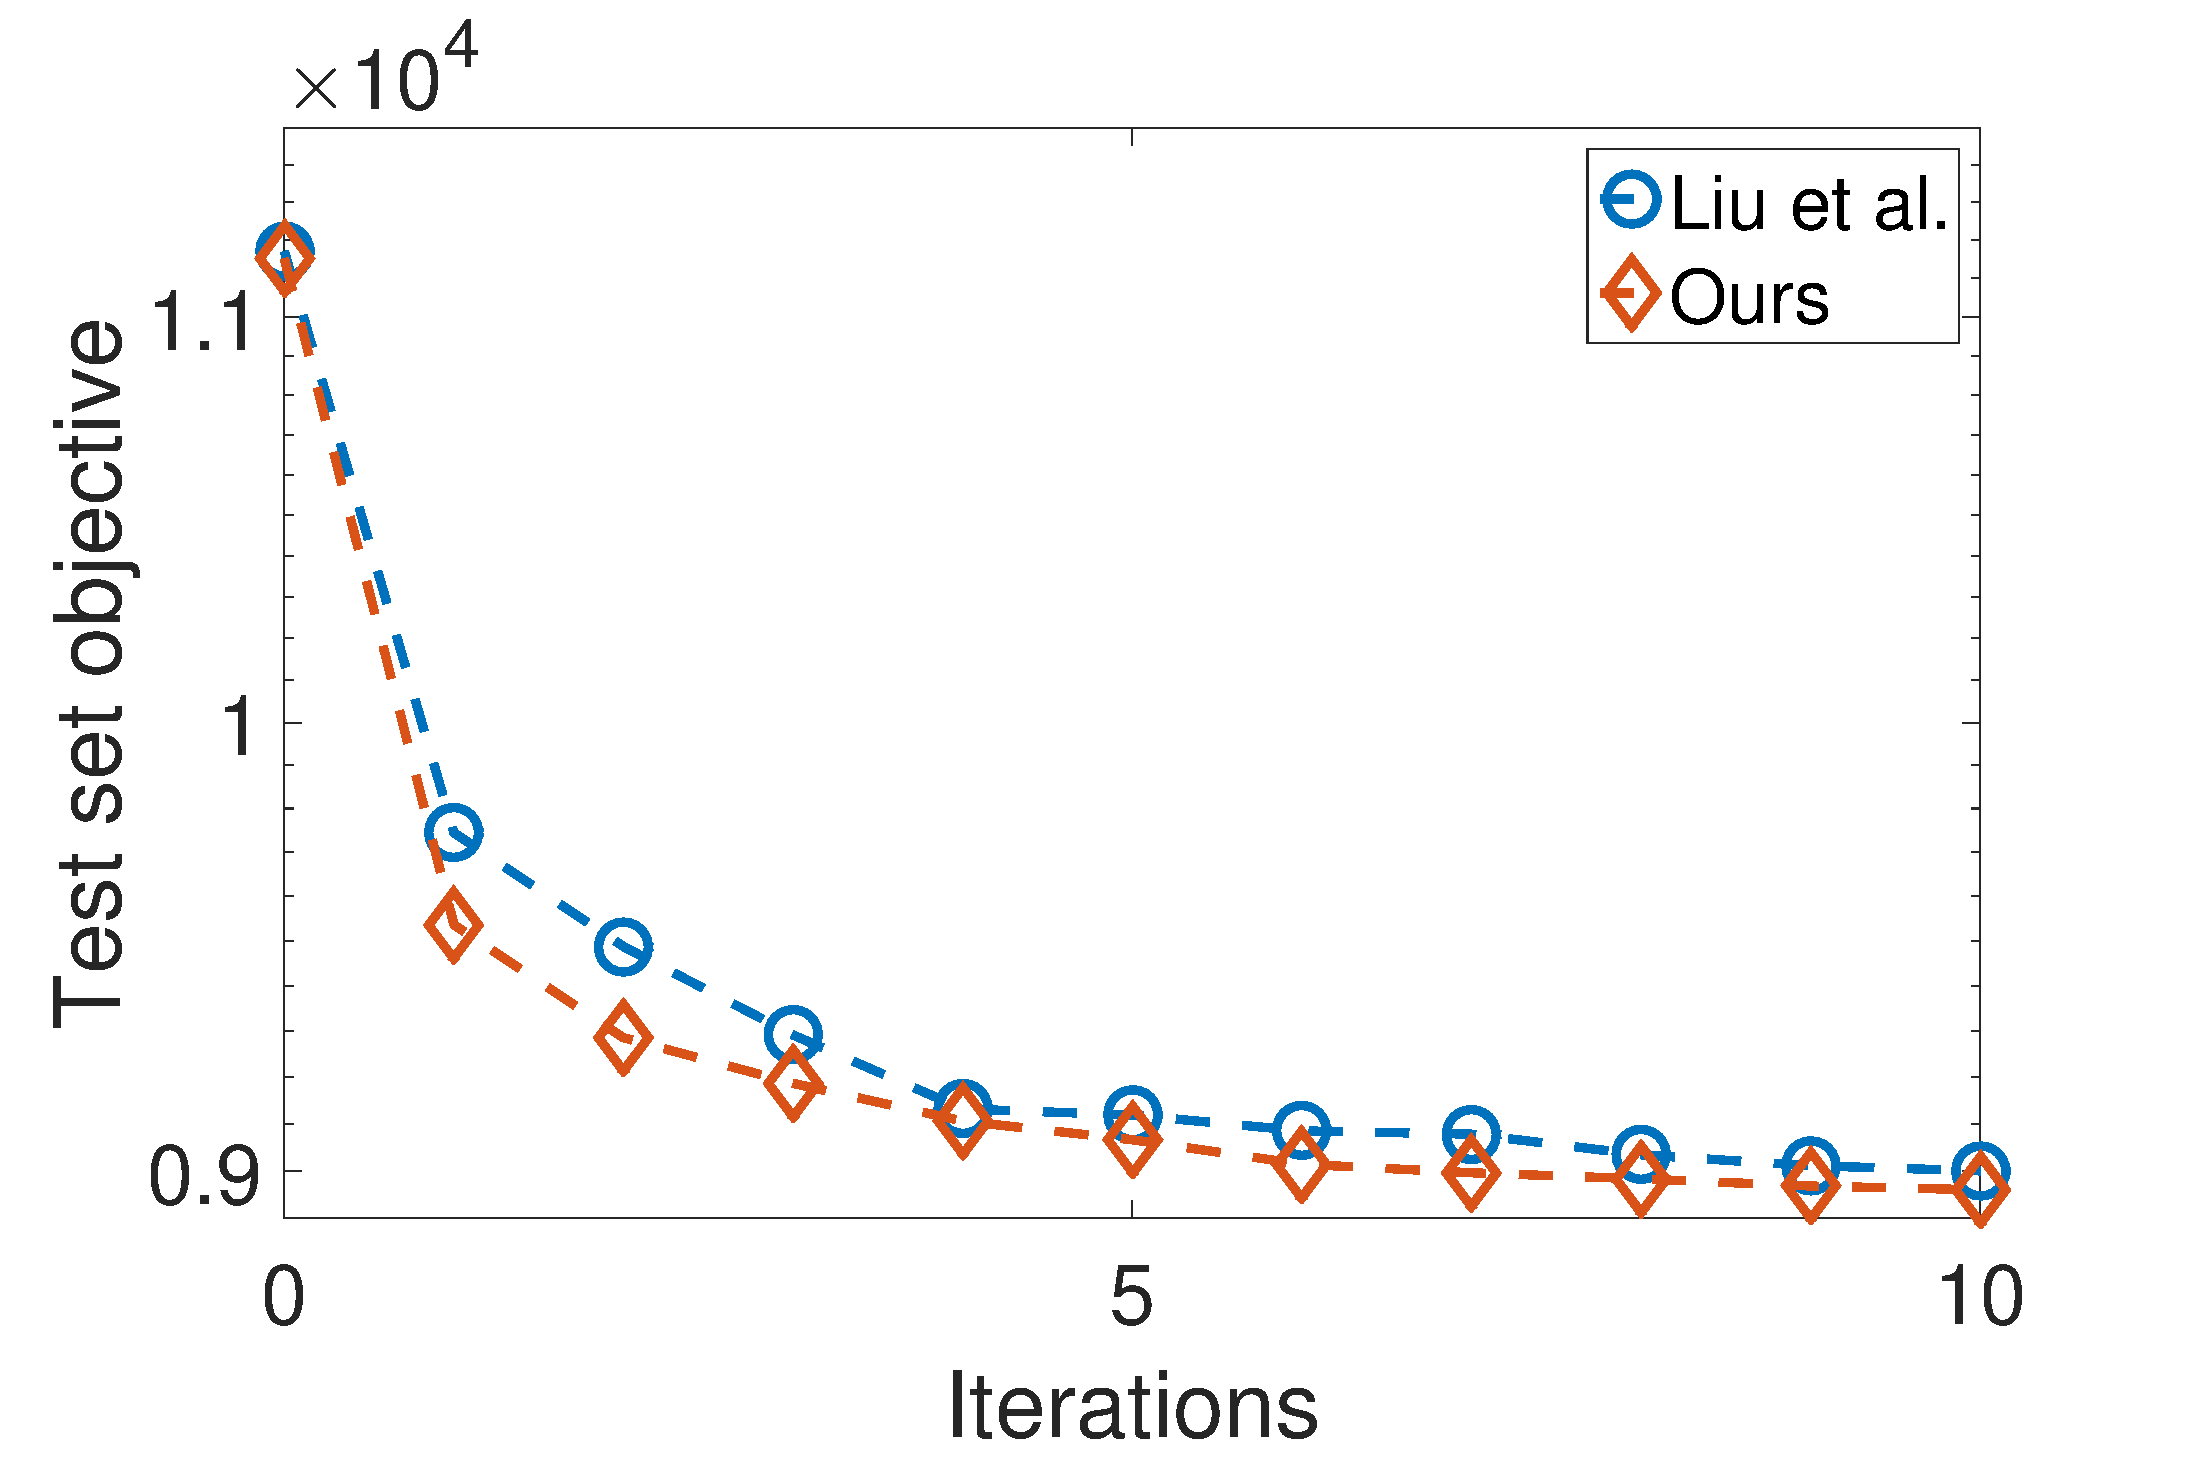
\includegraphics[width=1\linewidth]{figure/onlineVSliu-ite.pdf}
\end{subfigure}
\begin{subfigure}{0.45\textwidth}
  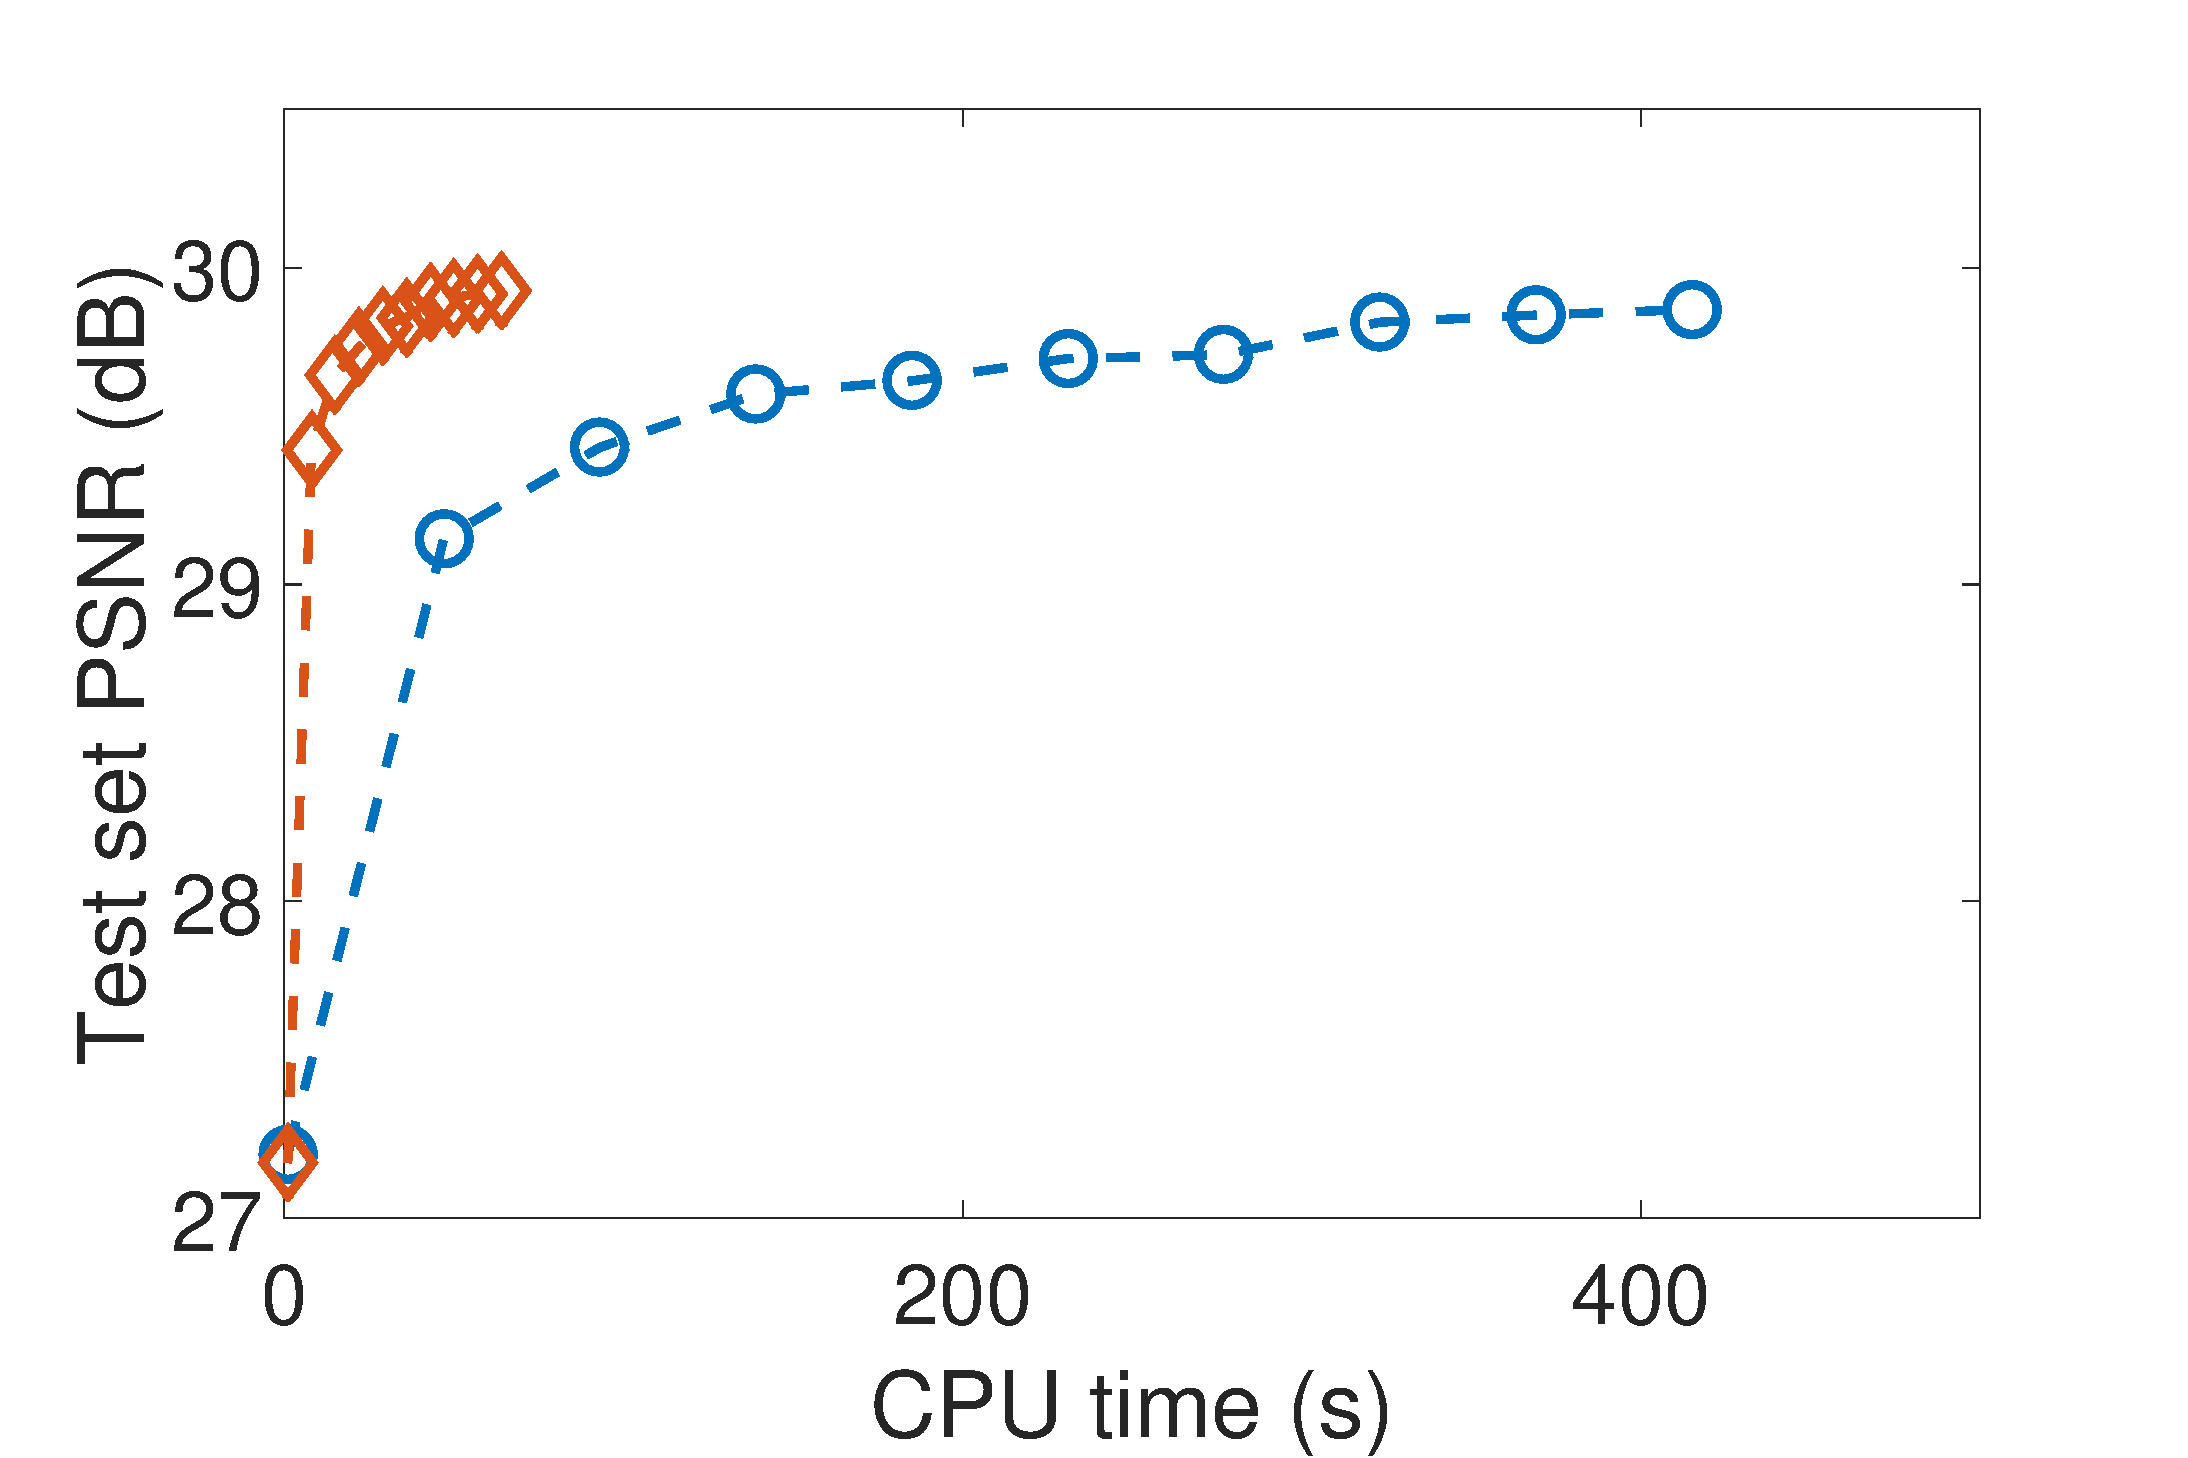
\includegraphics[width=1\linewidth]{figure/onlineVSliu-time.pdf}
\end{subfigure}

\caption{Experimental results obtained on city dataset. Top: Convergence of the test set objectives for our method (SOCSC) and the state-of-the-art online approach. Bottom: Testing PSNR with respect to execution time.}
\label{fig:onlineSmall-city}
\end{figure}

We then compare SOCSC with the state-of-the-art online algorithm on city dataset, the results of which are shown in Fig.\ \ref{fig:onlineSmall-city}. Similar to the results presented in Fig.~3 of the main manuscript, our method obtains comparable outcomes, meanwhile, achieves roughly $6 \times$ speedup.

\begin{figure*}[h]
\centering
  \begin{subfigure}{0.5\textwidth}
  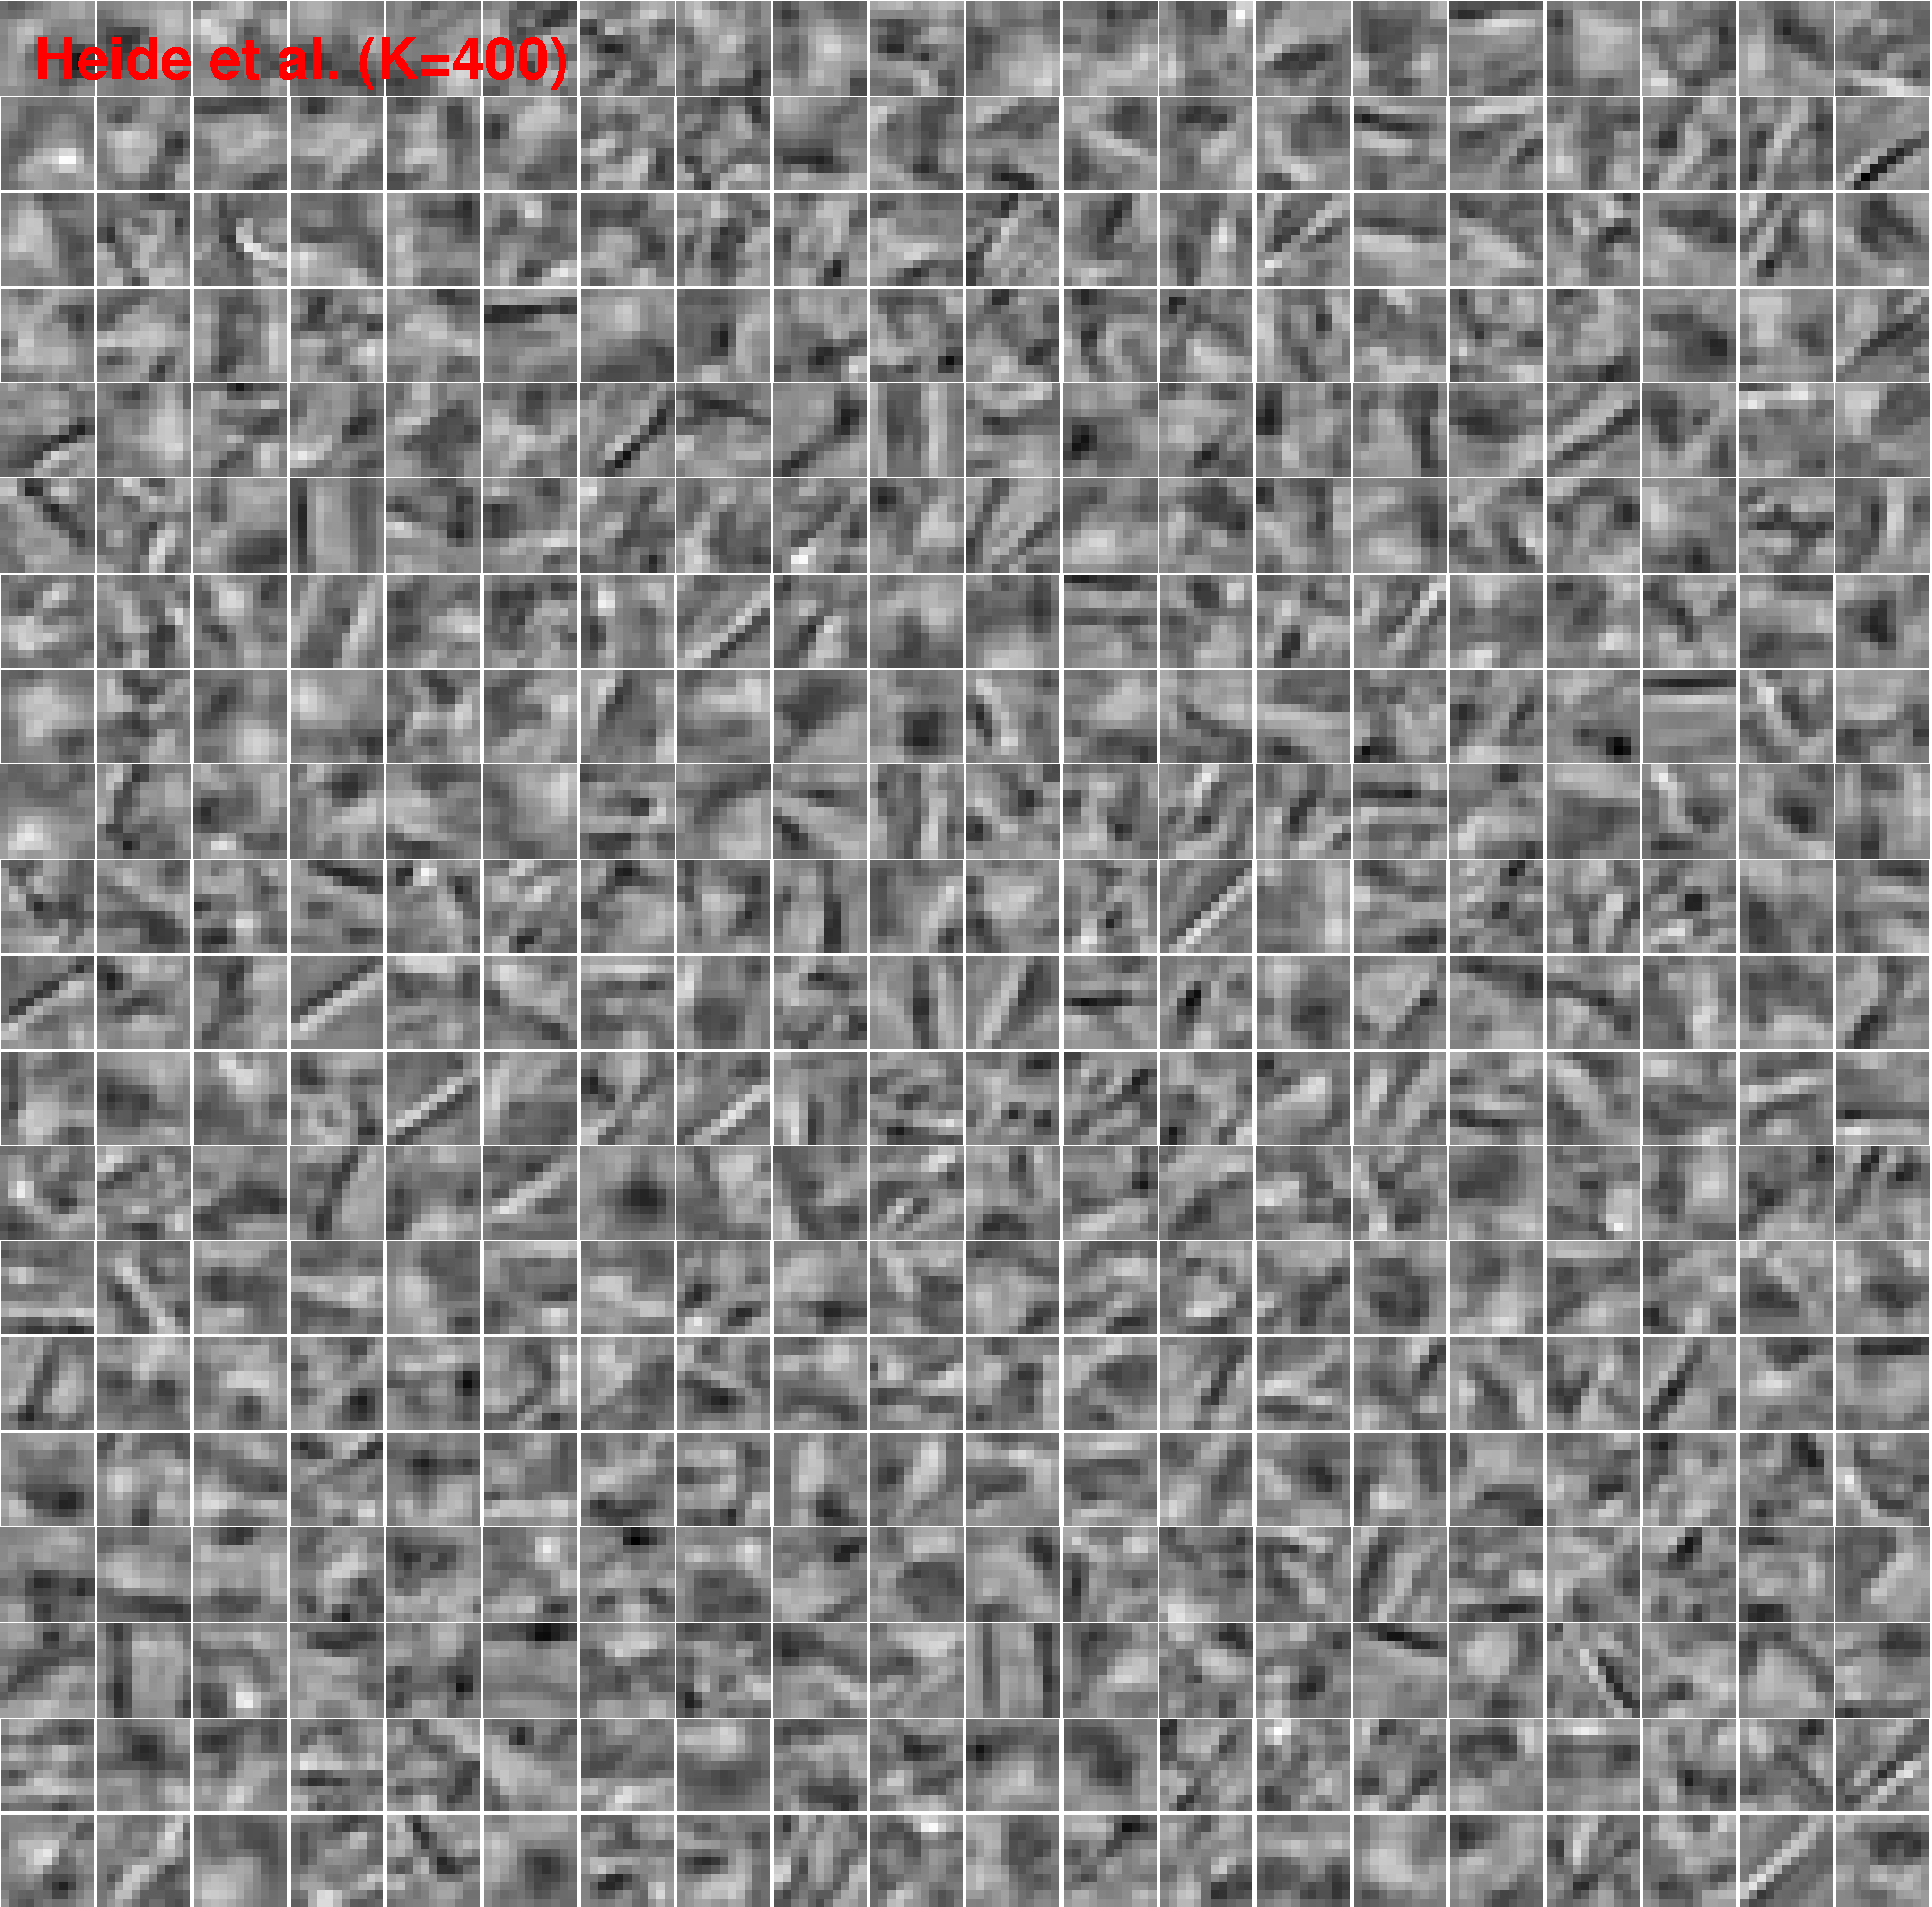
\includegraphics[width=1\linewidth]{figure/heide400-supple.pdf}
  \end{subfigure}
  \vspace{0.2cm}
  \begin{subfigure}{0.5\textwidth}
  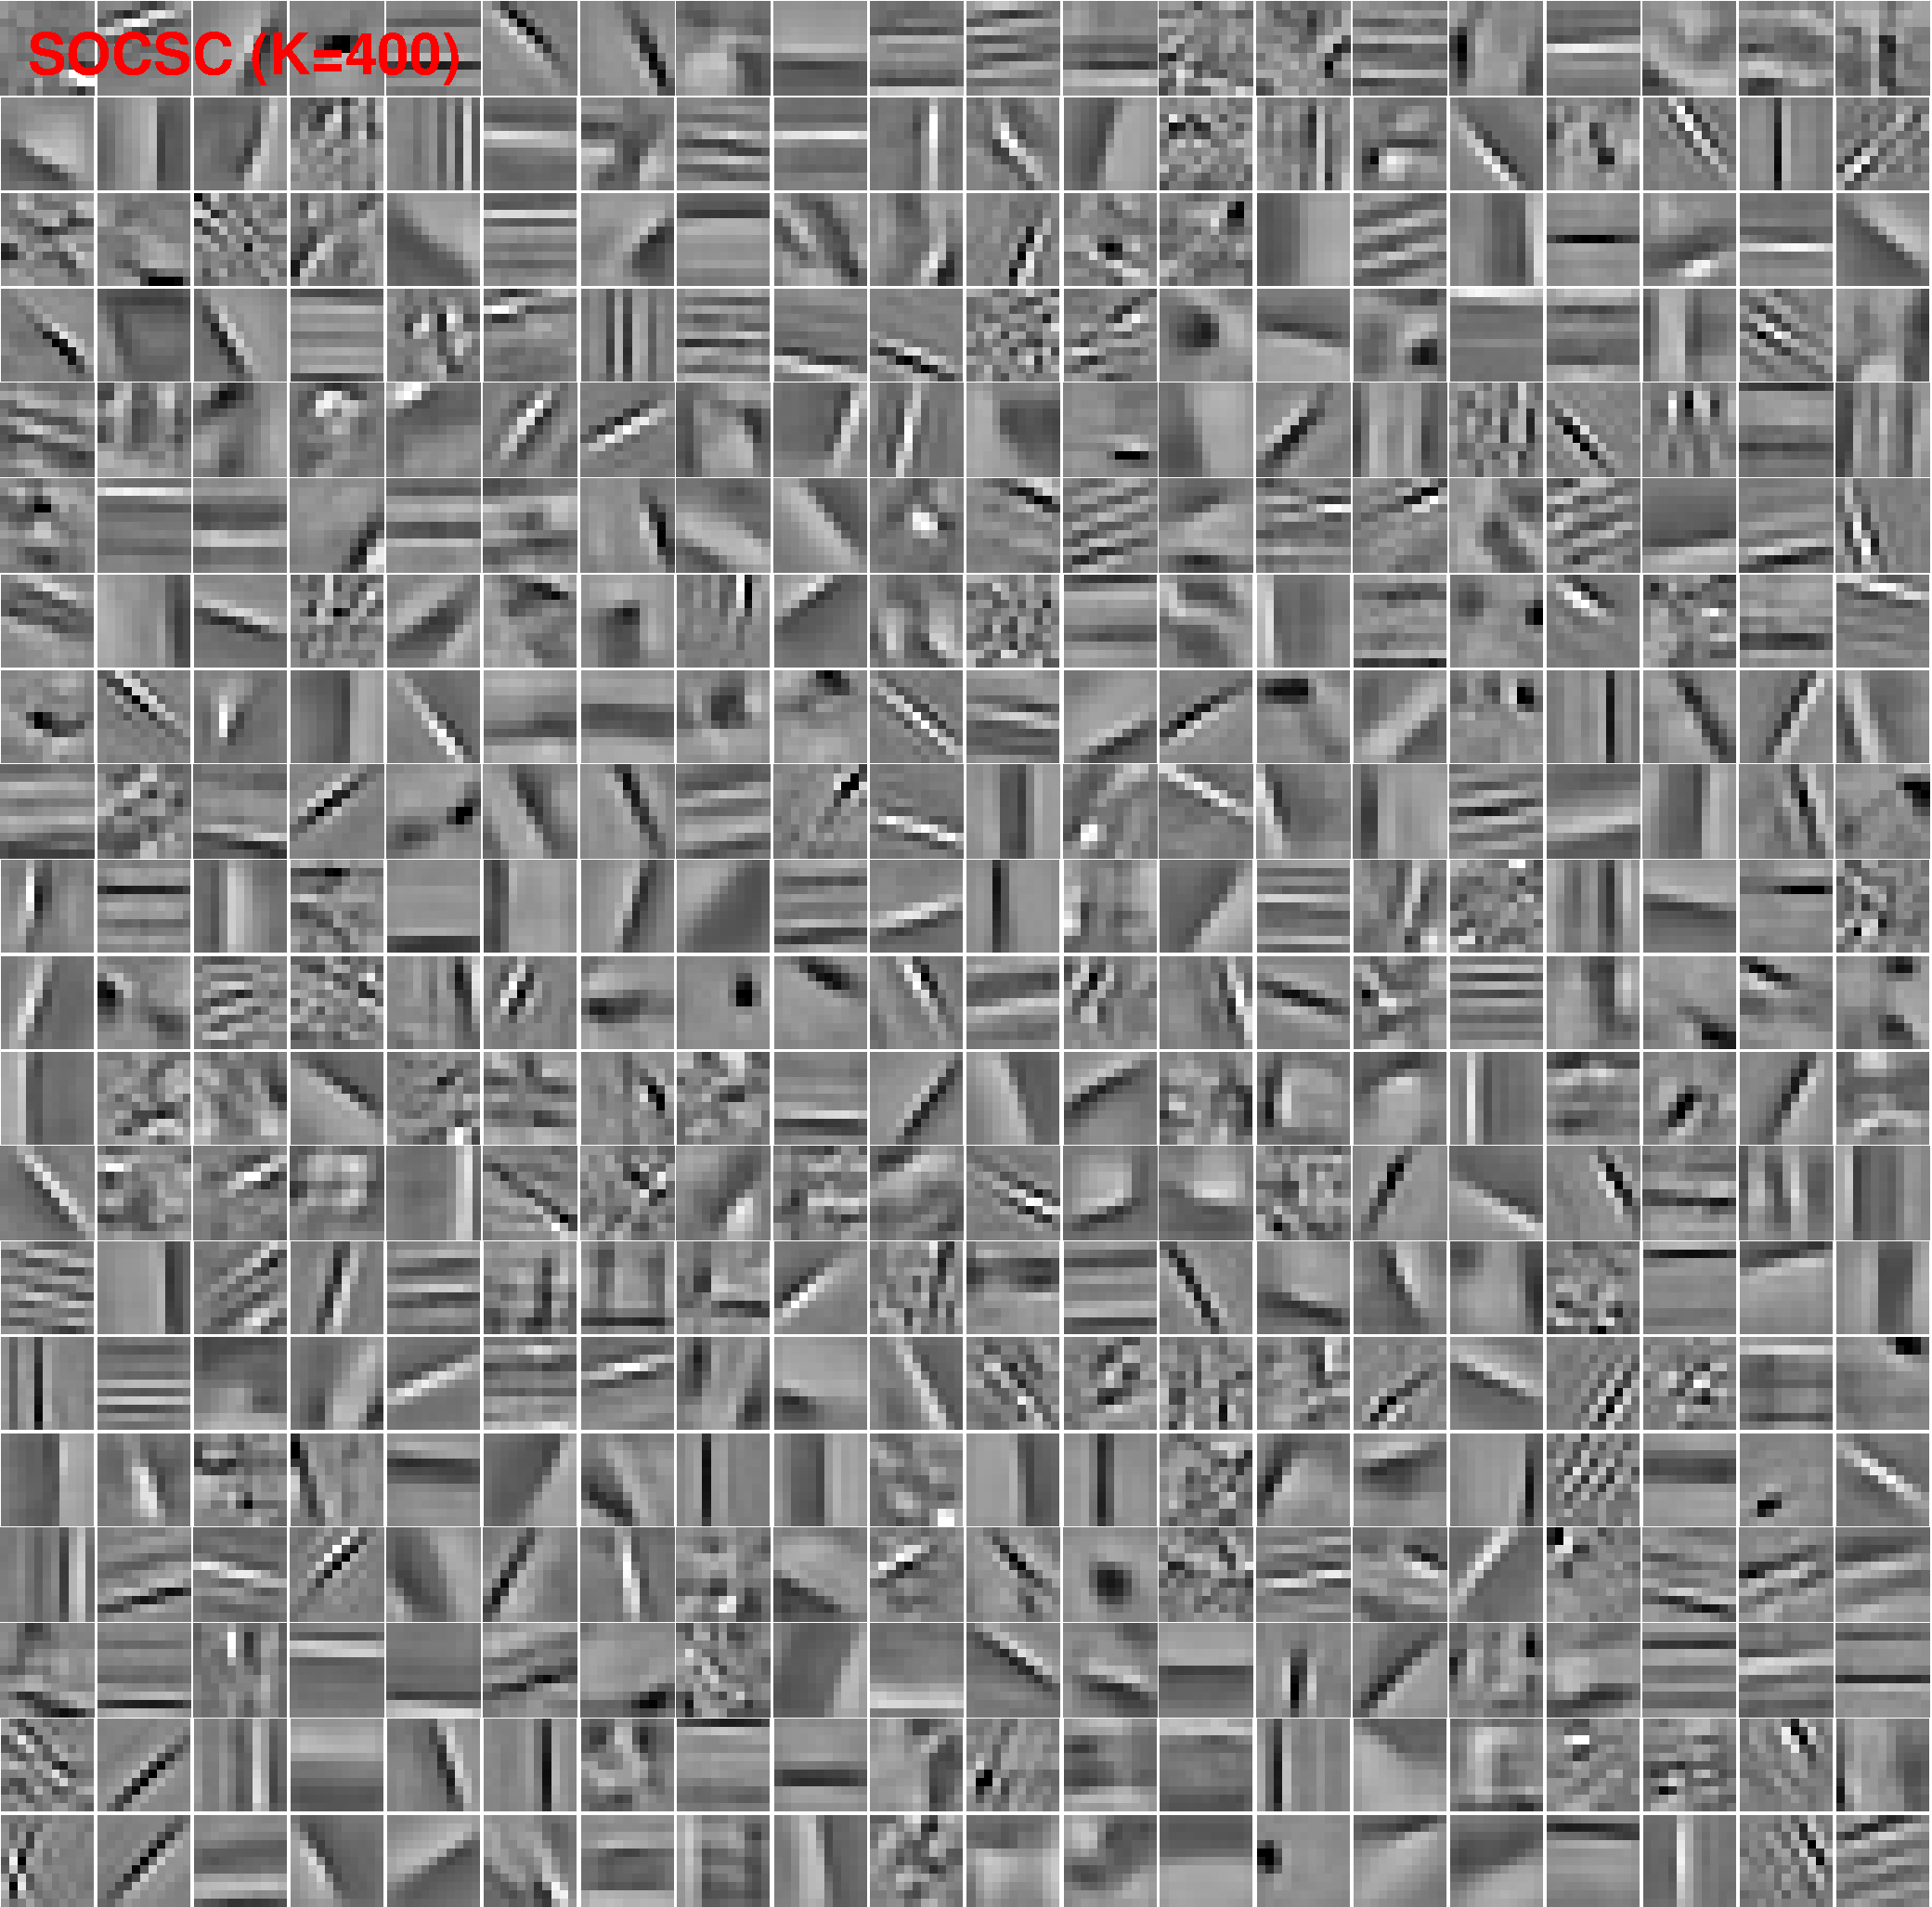
\includegraphics[width=1\linewidth]{figure/online400-supple.pdf}
  \end{subfigure}
  \vspace{0.2cm}

    \resizebox{0.8\linewidth}{!}{
        \begin{tabular}{|c||c|c|c|c|c|c|c|c|c|c|}
            \cline{1-11}
            Image & 1 & 2 & 3 & 4 & 5 & 6 & 7 & 8 & 9 & 10 \\
            \hline
            PSNR~[10] & 29.60 & 28.11 & 29.47 & 28.98 & 28.79 & 29.21 & 28.03  & 29.31 & 27.42 & 30.52 \\
            \hline
            PSNR ours & \textbf{30.24} & \textbf{28.34} & \textbf{29.95}  & \textbf{30.30} & \textbf{29.43} & \textbf{29.96} & \textbf{28.24} & \textbf{30.57} & \textbf{27.72} & \textbf{31.67} \\
            \hline
        \end{tabular} }
  \caption{ Visual and numerical comparisons between the learned over-complete dictionaries by batch-mode algorithm and by online-mode algorithm. Top: Over-complete dictionary learned by batch CSC model on small dataset, and proposed online CSC model (SOCSC) on large dataset. Bottom: Respective reconstruction quality for these two over-complete dictionaries applied for image inpainting.}
  \label{fig:overCompleteDic-dataset}
\end{figure*}

\section{Over-complete Dictionary and Large Datasets}

We verify the importance of a large dataset when learning the over-complete dictionary. in Fig.~\ref{fig:overCompleteDic-dataset}, we show a visual and quantitative comparisons between the over-complete dictionaries respectively learned by batch-mode algorithm on small dataset (the fruit dataset) and online-mode algorithm on large dataset (1000 images). Most of the filters learned from small dataset have poor structures and reveal very limited representative ability. The numerical results also demonstrate that it even shows a degraded reconstruction performance compared to the under-complete dictionary. Owing to plentiful training samples, our over-complete dictionary not only shows visually decent structures and more representative image features, but also leads to a significant improvement on image reconstruction. Based on all experimental results, it implies that the number of filters and number of training samples are both essential in the CSC model, therefore, the proposed algorithm has prominent advantages over the existing approaches.

\end{document} 